%! TEX program = lualatex
\documentclass[12pt,a4paper]{article} 

% Packages for formatting
\usepackage{fontspec}
\usepackage[ngerman]{babel}
\usepackage{geometry} 
\geometry{margin=1in} 
\usepackage{setspace} 
\usepackage{hyperref} 
\usepackage{xcolor}
\usepackage{amsmath} % for align*
\usepackage{amsthm} % neue Theorem-Umgebungen
\usepackage{enumitem} % für schöne Listen (Teilaufgaben)
\usepackage{mathbbol}
\usepackage{graphicx}
\usepackage{amssymb}
\usepackage{gensymb}

% Style settings
%\pagecolor{black}      % sets background color to black 
%\color{white}          % sets text color to white

% Change subsection to use a, b, c instead of 1, 2, 3
\renewcommand{\thesubsection}{\alph{subsection})} 

% Aufgaben-Umgebung definieren 
\newtheorem{aufgabe}{Aufgabe}

% Title page info 
\title{Blatt 01} 
\author{Hannes Rall \\ Albert-Ludwigs-University} 
\date{\today} 

\begin{document} 
% Title page 
\begin{titlepage}     
    \centering     
    \vspace*{2cm}     
    {\Huge\itshape Blatt 01\par}     
    \vspace{2cm}     
    {\Large\textsc{Hannes Rall}\par}     
    \vfill     
    {\large Albert-Ludwigs-University\\}     
    \vspace{1cm}     
    {\large\today\par}
\end{titlepage}

\newpage
\section*{Aufgabe 4}
Beweisen Sie unter Verwendung der Kongruenzsätze und Winkelsätzen an geschnittenen Parallelen:
\subsection*{(i)}
Seien g, h zwei parallele Geraden. Dann hat jeder Punkt $P\in g$ von h den gleichen Abstand.


    \centering        
    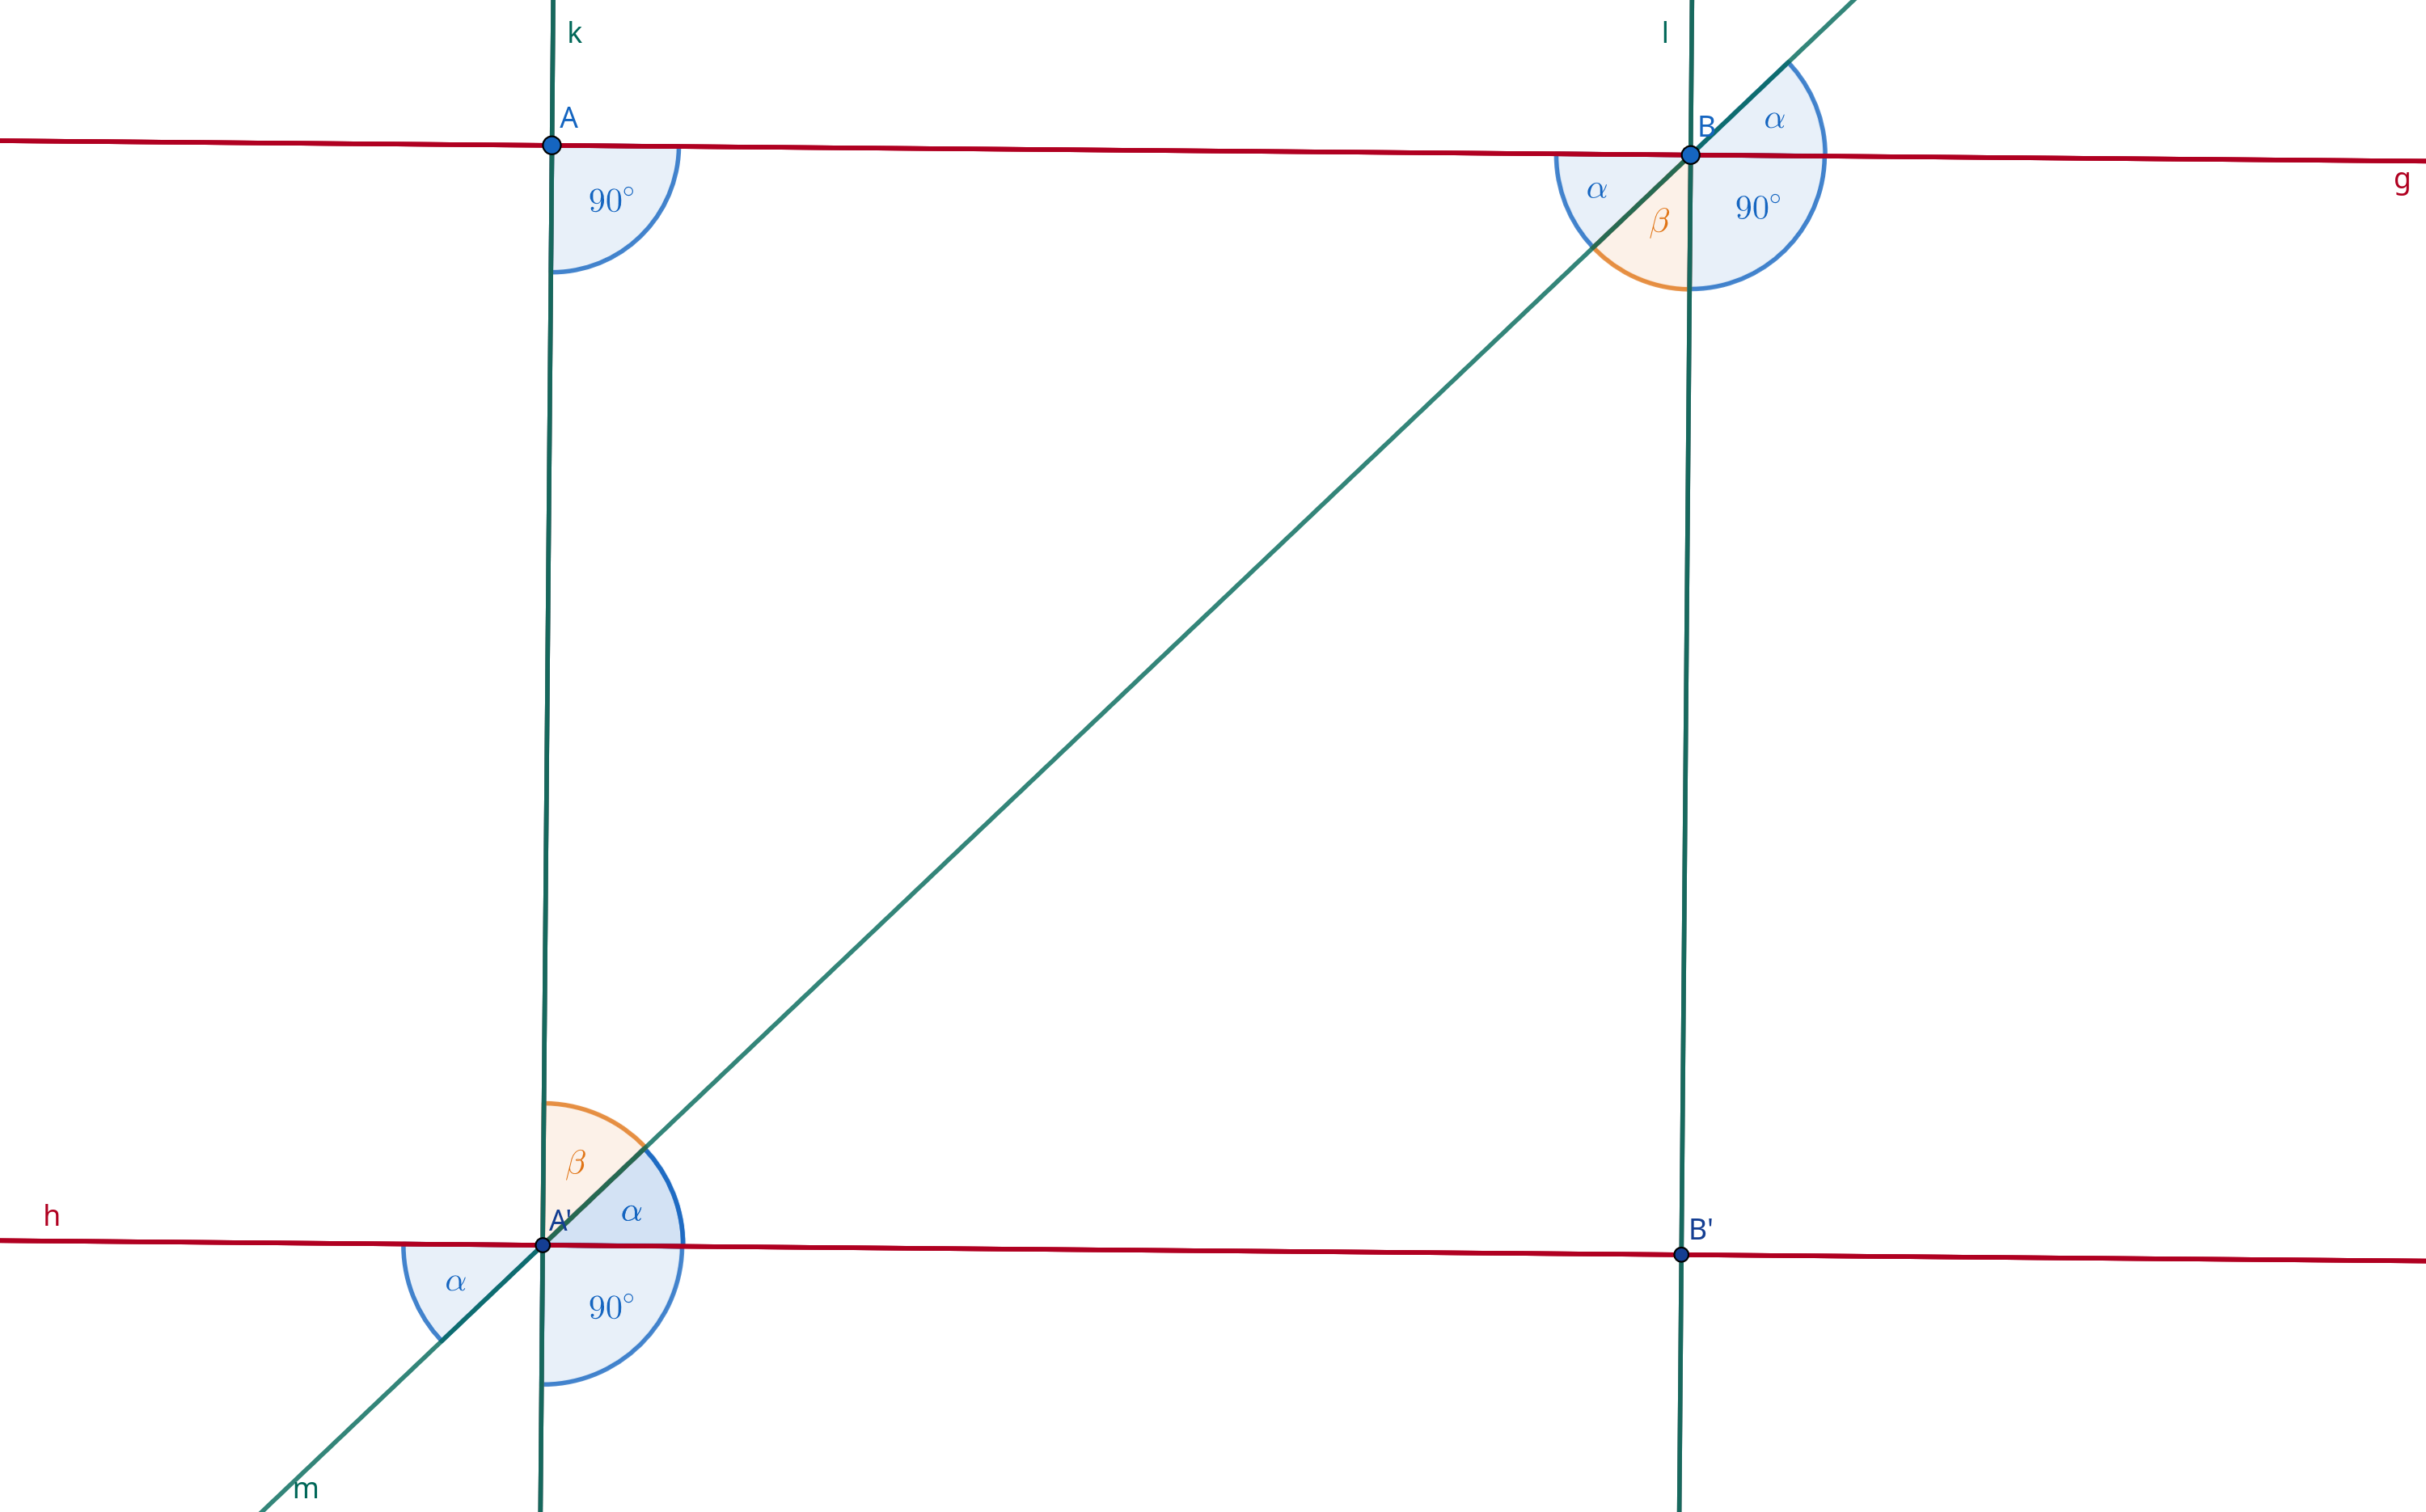
\includegraphics[width=0.8\textwidth]{Blatt_02_Aufgabe_1_i.png}
    \caption{Skizze}
    \label{fig:mein_bild}
\end{figure}
\noindent Beweis: \\
\\
\noindent Seien g und h zwei parallele Geraden. Seien A, B zwei Punkte auf g und sei A$\ne$B. Sei k die senkrechte Gerade zu g welche durch den Punkt A geht und sei l die senkrechte Gerade zu g welche durch den Punkt B geht. Da g, h parallel sind und k,l senkrecht auf g stehen, sind h,k und h, l nicht parallel. Somit schneiden sich h,k in einem Punkt und h,l in einem Punkt. Sei A' der Schnittpunkt von h und k und B' der Schnittpunkt von h und l. Außerdem sei m die Gerade durch A' und B.
\newline \\
Mit dem Stufenwinkelsatz folgt, dass k, l auch senkrecht auf h stehen. 
\newline \\
Sei $\alpha$ der Winkel $\angle BA'B'$. Nach Stufenwinkelsatz und Scheitelwinkelsatz (bzw. Wechselwinkelsatz) ist $\angle BA'B'= \angle A'BA$.\\
Sei $\beta$ der Winkel $\angle AA'B$. Nach Stufenwinkelsatz und Scheitelwinkelsatz (bzw. Wechselwinkelsatz) ist $\angle AA'B = \angle B'BA'$. \\
\\
Nun sind die Dreiecke $\triangle A'BA$ und $\triangle A'B'B$ nach WSW kongruent und |AA'| = |BB'|. Somit haben zwei beliebige (und deswegen alle) Punkte von g den gleichen Abstand zu h.

\newpage
\subsection*{(ii)}
Ein Parallelogramm ist per Definition ein Viereck, dessen gegenüberliegende Seiten parallel sind. Ein Viereck ist genau dann ein Parallelogramm, wenn die gegenüberliegenden Seiten gleich lang sind.

\noindent $\mathrm{Z\kern-.3em\raise-0.5ex\hbox{Z}}$ \\
(1) Wenn bei einem Viereck die gegenüberliegenden Seiten parallel sind, dann sind die gegenüberliegenden Seiten gleich lang.\\
(2) Wenn bei einem Viereck die gegenüberliegenden Seiten gleich lang sind, dann sind die gegenüberliegenden Seiten auch parallel.\\
Beweis (1):\\
\begin{figure}[htbp]
    \centering
    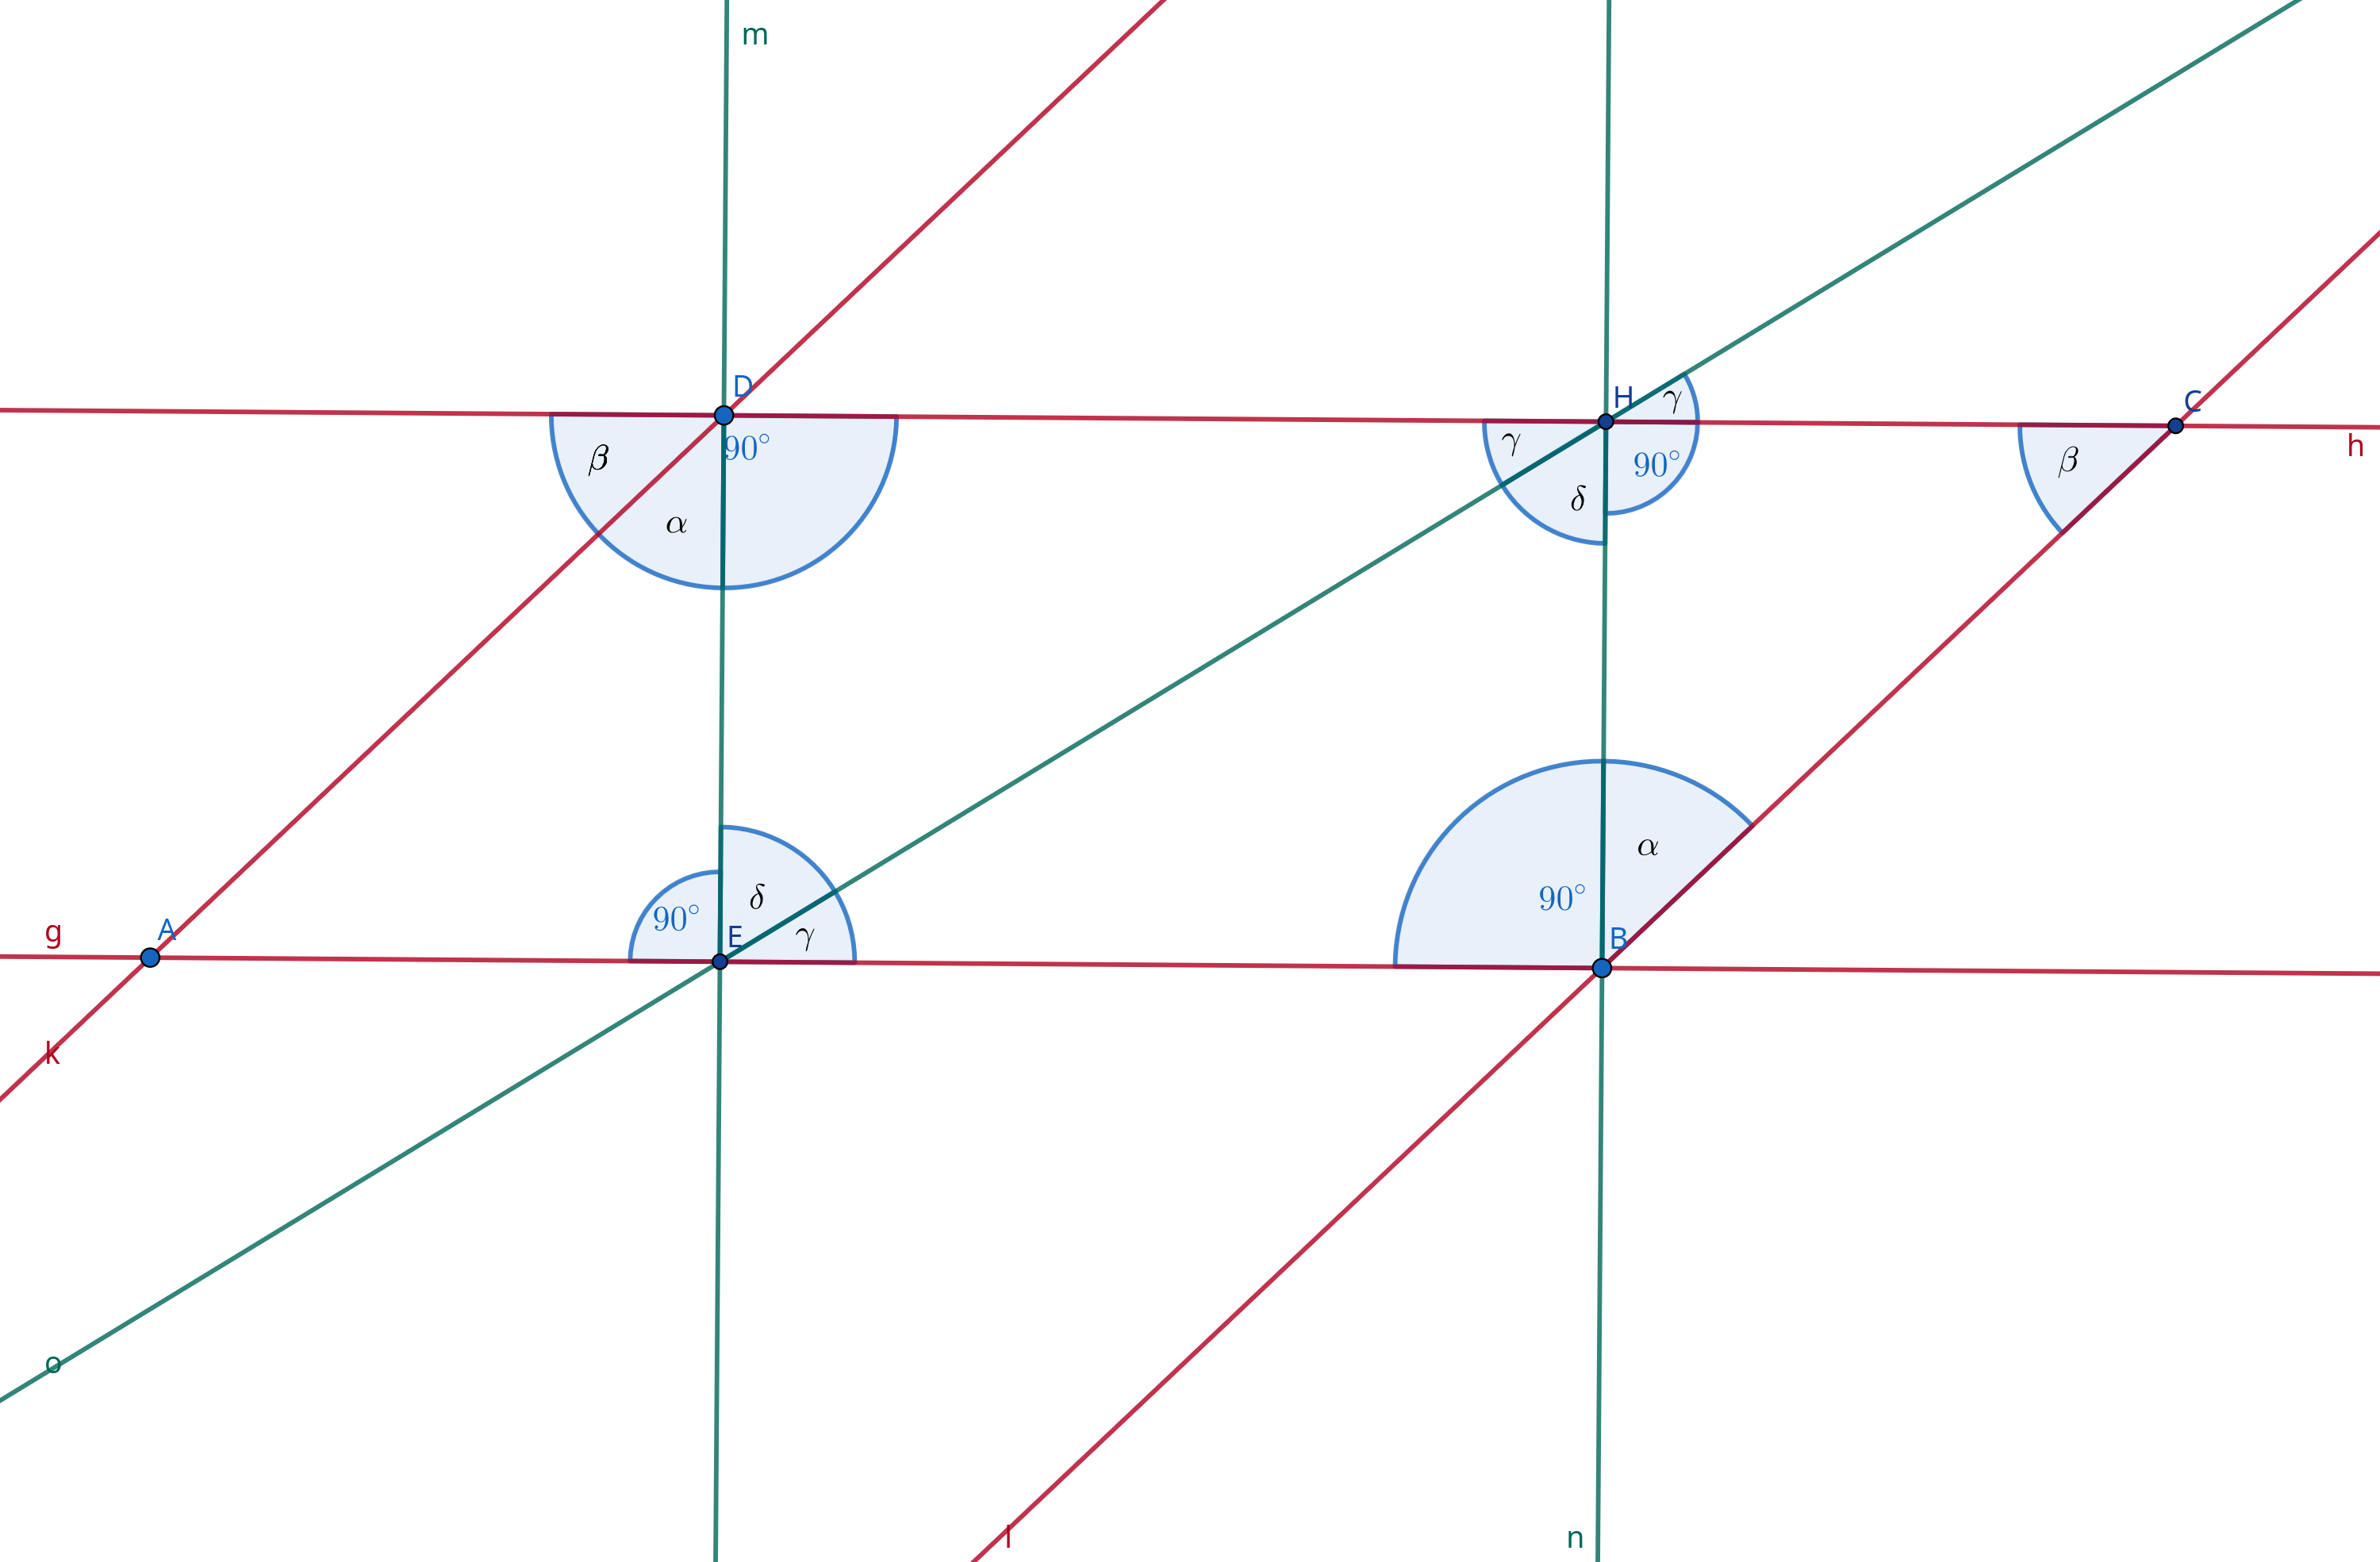
\includegraphics[width=0.8\textwidth]{Blatt_02_Aufgabe_1_ii.png}
    \caption{Skizze}
    \label{fig:mein_bild}
\end{figure} \\
Seien h und g parallele Geraden. Seien $D,C \in h$. Außerdem sei A ein Punkt auf g und k eine Gerade durch D und A. Sei l eine parallele Gerade zu k die durch den Punkt C geht. Da $l \parallel k$ und $k \nparallel g$ ist, ist auch $l \nparallel g$ und die Geraden l und g haben einen Schnittpunkt B. Somit ist $AD \parallel BC$ und $DC \parallel AB$. \\
Sei desweiteren m die senkrechte Gerade zu g, welche durch D geht und sei E der Schnittpunkt von m und g. Analog sei n die senkrechte Gerade zu h welche durch B geht und sei H der Schnittpunkt von h und n. Sei o die Gerade durch E und H.\\
Es gilt $\angle AED = \angle CHB = 90\degree$, da $m \perp g$ und $n \perp h$.\\
\\
Sei $\beta = \angle BCH$. Nach Stufenkwinkelsatz ist $\beta$ auch der Winkel, der von AD und h eingeschlossen wird. Sei $\alpha = \angle EDA$. Da $h \perp m$ ist $90\degree = \beta + \alpha$ bzw $\alpha = 90\degree - \beta$. Außerdem ist durch die Winkelsumme im Dreieck $\angle HBC = 90\degree - \beta = \alpha$. Da $m \perp h$ ist $d(D, g) = d(E, h) = |DE|$. Analog ist $d(H, g) = d(B, h) = |HB|$. Mit Aufgabenteil (i) folgt, dass $|DE| = d(D,g) = d(H, g) = |HB|$. Somit sind die Dreiecke $\triangle AED$ und $\triangle BCH$ nach WSW kongruent und |AD| = |BC|.\\
\newpage

\noindent Nun ist nach Stufenwinkelsatz und Scheitelwinkelsatz $\gamma = \angle HEB = \angle EHD$ durch die Winkelsumme im Dreieck folgt $\delta = \angle DEH = \angle BHE$. Durch WSW Also sind die Dreiecke $\triangle BHE$ und $\triangle EHD$ kongruent nach WSW, also |DH| = |EB|.\\
\\
Beweis (2): \\
\newpage
\section*{Aufgabe 5}
\subsection*{(i)}
\begin{figure}[htbp]             
    \centering             
    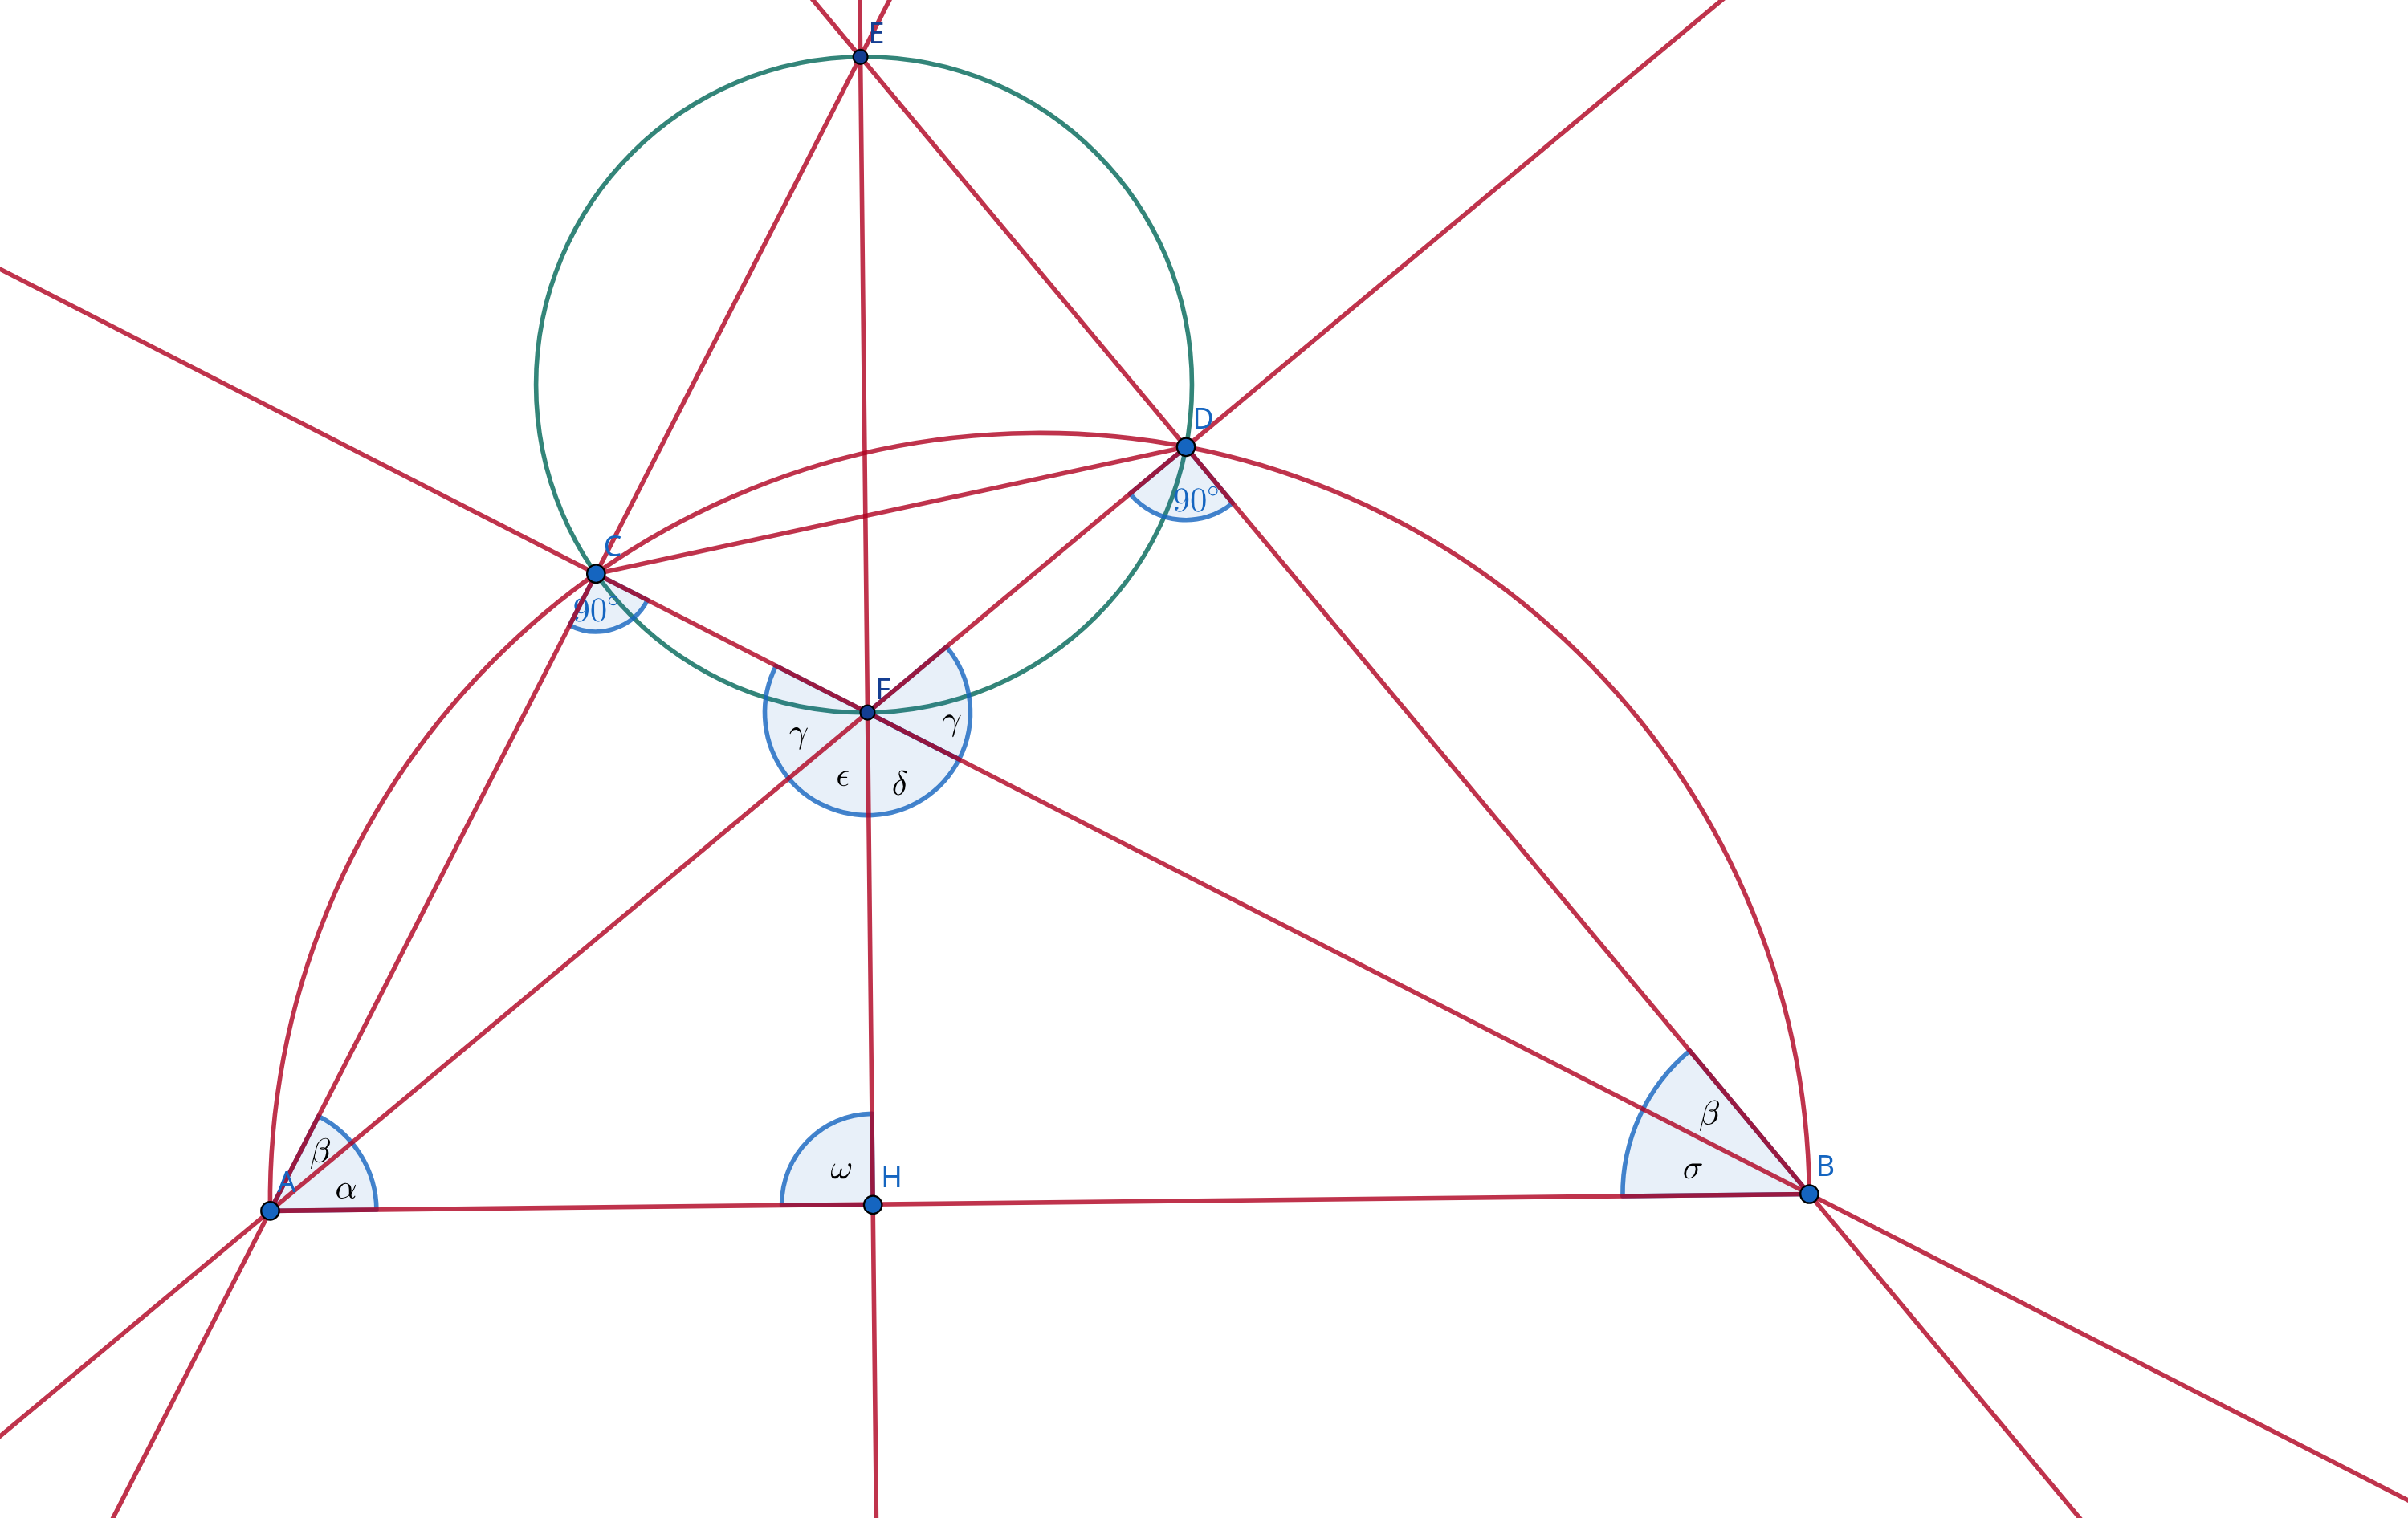
\includegraphics[width=0.8\textwidth]{Blatt_02_Aufgabe_2_i.png}
    \caption{Skizze}     
    \label{fig:mein_bild}
\end{figure}
\noindent Sei k ein Halbkreis über einer Strecke AB. Seien C, D zwei verschiedene Punkte auf k. Die Geraden durch AC und BD schneiden sich in einem Punkt E und die Geraden durch AD und BC schneiden sich in einem Punkt F.\\
\\
\noindent $\mathrm{Z\kern-.3em\raise-0.5ex\hbox{Z}}$ 
Die Gerade durch E und F steht senkrecht auf AB.\\
\\
Beweis: \\
Durch den Satz von Thales wissen wir, dass $\angle BCA = 90\degree$. Analog ist $\angle BDA = 90\degree$. Außerdem folgt mit dem Nebenwinkelsatz, dass $\angle ECF = 180\degree - 90\degree = 90\degree$. Analog folgt $\angle FDE = 90\degree$. Mit der Umkehrung vom Satz von Thales, folgt das EF der Durchmesser des Umkreises von $\triangle CFE$ und $\triangle FDE$ ist. Daraus wiederum folgt, das $CFDE$ ein Sehnenviereck ist. 
\newpage
\section*{Aufgabe 6}
\subsection*{(i)}
Bei einem Rechteck sind die beiden Diagonalen gleich lang und sie schneiden sich genau in der Mitte. Dieser Schnittpunkt ist von allen vier Ecken gleich weit entfernt. Wenn man einen Kreis um diesen Punkt mit dem Radius bis zu einer Ecke zeichnet, so liegen alle vier Ecken des Rechtecks auf diesem Kreis. Deshalb hat jedes Rechteck einen Umkreis. Man kann außerdem mit der Hilfe von kongruenten Dreiecken zeigen, dass die Diagonalen gleich lang sein müssen. Bzw man kann auch den Satz des Pythagoras verwenden um das zu zeigen.\\

\subsection*{(ii)}
Ein Viereck besitzt genau dann einen Umkreis, wenn sich alle vier Mittelsenkrechten in einem Punkt schneiden. Dieser Schnittpunkt ist dann automatisch Mittelpunkt des Umkreises.  Solche Vierecke heißen \emph{Sehnenvierecke}. Ein Viereck ist genau dann ein Sehnenviereck, wenn die Summen der gegenüberliegenden Innenwinkel jeweils $180^\circ$ ergeben, also $\alpha + \gamma = \beta + \delta = 180^\circ$. \\

\subsection*{(iii)}
Besondere Vierecke mit Umkreis:\\
\begin{itemize}
    \item \textbf{Quadrat:} Ein Quadrat ist ein Rechteck mit vier gleich langen Seiten. Die Diagonalen sind gleich lang und schneiden sich im Mittelpunkt. Daher gibt es immer einen Umkreis.
    \item \textbf{Gleichschenkliges Trapez:} Ein gleichschenkliges Trapez hat zwei gleich lange Schenkel und die Diagonalen sind gleich lang. Deshalb kann man auch hier einen Umkreis zeichnen.
\end{itemize}     

\newpage
\subsection*{(iv)}
Fiktives Gespräch – Lernförderliche Weiterführung:
\begin{quote}
    „Ihr habt schon gesehen, dass Rechtecke und Quadrate immer einen Umkreis haben. Aber auch manche Trapeze, nämlich die gleichschenkligen, haben einen Umkreis.\\
    Nicht jedes Viereck hat einen Umkreis. Zum Beispiel ein normales Parallelogramm oder ein beliebiges Trapez ohne gleich lange Schenkel – da kann man keinen Umkreis zeichnen.\\
Ein Viereck hat genau dann einen Umkreis, wenn die Summen der gegenüberliegenden Winkel $180^\circ$ ergeben bzw wenn sich die Mittelsenkrechten aller vier Seiten in einem Punkt schneiden. Das ist bei Rechtecken, Quadraten und gleichschenkligen Trapezen der Fall!“
\end{quote}     

\subsection*{(v)}
Das gilt nur bei Rechtecken im Allgemeinen. Bei diesen Vierecken schneiden sich die Diagonalen in der Mitte und dieser Punkt ist der Mittelpunkt des Umkreises. Bei anderen Vierecken (z.\,B. gleichschenkligen Trapezen) liegt der Mittelpunkt des Umkreises nicht unbedingt im Schnittpunkt der Diagonalen. Anschaulich begründen kann man das auch, indem man ein Rechteck in Geogebra zeichnet und den Umkreis konstruiert. Dann verschiebt man Ecken auf dem Kreis. Offensichtlich besitzt das Vierreck immernoch einen Umkreis aber die Diagonalen schneiden nicht unbedingt den Mittelpunkt.
\end{document}
